\PassOptionsToPackage{round}{natbib}
\documentclass[notoc]{tufte-book}
\setcounter{tocdepth}{2}
\hypersetup{colorlinks}% uncomment this line if you prefer colored hyperlinks (e.g., for onscreen viewing)

%%
% Book metadata
\title{Deep Learning}
\author[Aakash Ghosh\\19MS129]{Aakash Ghosh }
\publisher{Written for the completion of Independent Study under Dr. Dwaipayan Roy}

%%
% If they're installed, use Bergamo and Chantilly from www.fontsite.com.
% They're clones of Bembo and Gill Sans, respectively.
%\IfFileExists{bergamo.sty}{\usepackage[osf]{bergamo}}{}% Bembo
%\IfFileExists{chantill.sty}{\usepackage{chantill}}{}% Gill Sans

%\usepackage{microtype}

%%
% Just some sample text
\usepackage{lipsum}

%%
% For nicely typeset tabular material
\usepackage{booktabs}

%%
% For graphics / images
\usepackage{graphicx}
\setkeys{Gin}{width=\linewidth,totalheight=\textheight,keepaspectratio}
\graphicspath{{graphics/}}

% The fancyvrb package lets us customize the formatting of verbatim
% environments.  We use a slightly smaller font.
\usepackage{fancyvrb}
\fvset{fontsize=\normalsize}

%%
% Prints argument within hanging parentheses (i.e., parentheses that take
% up no horizontal space).  Useful in tabular environments.
\newcommand{\hangp}[1]{\makebox[0pt][r]{(}#1\makebox[0pt][l]{)}}

%%
% Prints an asterisk that takes up no horizontal space.
% Useful in tabular environments.
\newcommand{\hangstar}{\makebox[0pt][l]{*}}

%%
% Prints a trailing space in a smart way.
\usepackage{xspace}

%%
% Some shortcuts for Tufte's book titles.  The lowercase commands will
% produce the initials of the book title in italics.  The all-caps commands
% will print out the full title of the book in italics.
\newcommand{\vdqi}{\textit{VDQI}\xspace}
\newcommand{\ei}{\textit{EI}\xspace}
\newcommand{\ve}{\textit{VE}\xspace}
\newcommand{\be}{\textit{BE}\xspace}
\newcommand{\VDQI}{\textit{The Visual Display of Quantitative Information}\xspace}
\newcommand{\EI}{\textit{Envisioning Information}\xspace}
\newcommand{\VE}{\textit{Visual Explanations}\xspace}
\newcommand{\BE}{\textit{Beautiful Evidence}\xspace}

\newcommand{\TL}{Tufte-\LaTeX\xspace}

% Prints the month name (e.g., January) and the year (e.g., 2008)
\newcommand{\monthyear}{%
  \ifcase\month\or January\or February\or March\or April\or May\or June\or
  July\or August\or September\or October\or November\or
  December\fi\space\number\year
}


% Prints an epigraph and speaker in sans serif, all-caps type.
\newcommand{\openepigraph}[2]{%
  %\sffamily\fontsize{14}{16}\selectfont
  \begin{fullwidth}
  \sffamily\large
  \begin{doublespace}
  \noindent\allcaps{#1}\\% epigraph
  \noindent\allcaps{#2}% author
  \end{doublespace}
  \end{fullwidth}
}

% Inserts a blank page
\newcommand{\blankpage}{\newpage\hbox{}\thispagestyle{empty}\newpage}

\usepackage{units}

% Typesets the font size, leading, and measure in the form of 10/12x26 pc.
\newcommand{\measure}[3]{#1/#2$\times$\unit[#3]{pc}}

% Macros for typesetting the documentation
\newcommand{\hlred}[1]{\textcolor{Maroon}{#1}}% prints in red
\newcommand{\hangleft}[1]{\makebox[0pt][r]{#1}}
\newcommand{\hairsp}{\hspace{1pt}}% hair space
\newcommand{\hquad}{\hskip0.5em\relax}% half quad space
\newcommand{\TODO}{\textcolor{red}{\bf TODO!}\xspace}
\newcommand{\na}{\quad--}% used in tables for N/A cells
\providecommand{\XeLaTeX}{X\lower.5ex\hbox{\kern-0.15em\reflectbox{E}}\kern-0.1em\LaTeX}
\newcommand{\tXeLaTeX}{\XeLaTeX\index{XeLaTeX@\protect\XeLaTeX}}
% \index{\texttt{\textbackslash xyz}@\hangleft{\texttt{\textbackslash}}\texttt{xyz}}
\newcommand{\tuftebs}{\symbol{'134}}% a backslash in tt type in OT1/T1
\newcommand{\doccmdnoindex}[2][]{\texttt{\tuftebs#2}}% command name -- adds backslash automatically (and doesn't add cmd to the index)
\newcommand{\doccmddef}[2][]{%
  \hlred{\texttt{\tuftebs#2}}\label{cmd:#2}%
  \ifthenelse{\isempty{#1}}%
    {% add the command to the index
      \index{#2 command@\protect\hangleft{\texttt{\tuftebs}}\texttt{#2}}% command name
    }%
    {% add the command and package to the index
      \index{#2 command@\protect\hangleft{\texttt{\tuftebs}}\texttt{#2} (\texttt{#1} package)}% command name
      \index{#1 package@\texttt{#1} package}\index{packages!#1@\texttt{#1}}% package name
    }%
}% command name -- adds backslash automatically
\newcommand{\doccmd}[2][]{%
  \texttt{\tuftebs#2}%
  \ifthenelse{\isempty{#1}}%
    {% add the command to the index
      \index{#2 command@\protect\hangleft{\texttt{\tuftebs}}\texttt{#2}}% command name
    }%
    {% add the command and package to the index
      \index{#2 command@\protect\hangleft{\texttt{\tuftebs}}\texttt{#2} (\texttt{#1} package)}% command name
      \index{#1 package@\texttt{#1} package}\index{packages!#1@\texttt{#1}}% package name
    }%
}% command name -- adds backslash automatically
\newcommand{\docopt}[1]{\ensuremath{\langle}\textrm{\textit{#1}}\ensuremath{\rangle}}% optional command argument
\newcommand{\docarg}[1]{\textrm{\textit{#1}}}% (required) command argument
\newenvironment{docspec}{\begin{quotation}\ttfamily\parskip0pt\parindent0pt\ignorespaces}{\end{quotation}}% command specification environment
\newcommand{\docenv}[1]{\texttt{#1}\index{#1 environment@\texttt{#1} environment}\index{environments!#1@\texttt{#1}}}% environment name
\newcommand{\docenvdef}[1]{\hlred{\texttt{#1}}\label{env:#1}\index{#1 environment@\texttt{#1} environment}\index{environments!#1@\texttt{#1}}}% environment name
\newcommand{\docpkg}[1]{\texttt{#1}\index{#1 package@\texttt{#1} package}\index{packages!#1@\texttt{#1}}}% package name
\newcommand{\doccls}[1]{\texttt{#1}}% document class name
\newcommand{\docclsopt}[1]{\texttt{#1}\index{#1 class option@\texttt{#1} class option}\index{class options!#1@\texttt{#1}}}% document class option name
\newcommand{\docclsoptdef}[1]{\hlred{\texttt{#1}}\label{clsopt:#1}\index{#1 class option@\texttt{#1} class option}\index{class options!#1@\texttt{#1}}}% document class option name defined
\newcommand{\docmsg}[2]{\bigskip\begin{fullwidth}\noindent\ttfamily#1\end{fullwidth}\medskip\par\noindent#2}
\newcommand{\docfilehook}[2]{\texttt{#1}\index{file hooks!#2}\index{#1@\texttt{#1}}}
\newcommand{\doccounter}[1]{\texttt{#1}\index{#1 counter@\texttt{#1} counter}}









\definecolor{ch}{RGB}{60,72,107}
\definecolor{sec}{RGB}{200,75,49}
\definecolor{subsec}{RGB}{244,80,80}









% add numbers to chapters, sections, subsections
\setcounter{secnumdepth}{2}

% chapter format
\titleformat{\chapter}%
  {\huge\rmfamily\itshape\color{ch}}% format applied to label+text
  {\llap{\colorbox{ch}{\parbox{1.5cm}{\hfill\itshape\huge\color{white}\thechapter}}}}% label
  {2pt}% horizontal separation between label and title body
  {}% before the title body
  []% after the title body

% section format
\titleformat{\section}%
  {\normalfont\Large\itshape\color{sec}}% format applied to label+text
  {\llap{\colorbox{sec}{\parbox{1.5cm}{\hfill\color{white}\thesection}}}}% label
  {1em}% horizontal separation between label and title body
  {}% before the title body
  []% after the title body

% subsection format
\titleformat{\subsection}%
  {\normalfont\large\itshape\color{subsec}}% format applied to label+text
  {\llap{\colorbox{subsec}{\parbox{1.5cm}{\hfill\color{white}\thesubsection}}}}% label
  {1em}% horizontal separation between label and title body
  {}% before the title body
  []% after the title body

\usepackage{physics}
\usepackage{amsmath}
\usepackage{tikz}
\usepackage{mathdots}
\usepackage{yhmath}
\usepackage{cancel}
\usepackage{color}
\usepackage{siunitx}
\usepackage{array}
\usepackage{multirow}
\usepackage{amssymb}
\usepackage{gensymb}
\usepackage{tabularx}
\usepackage{extarrows}
\usepackage{booktabs}
\usetikzlibrary{fadings}
\usetikzlibrary{patterns}
\usetikzlibrary{shadows.blur}
\usetikzlibrary{shapes}




\usepackage{listings}


\definecolor{dkgreen}{rgb}{0,0.6,0}
\definecolor{gray}{rgb}{0.5,0.5,0.5}
\definecolor{mauve}{rgb}{0.58,0,0.82}

\lstset{frame=tb,
  language=Python,
  aboveskip=3mm,
  belowskip=3mm,
  showstringspaces=false,
  columns=flexible,
  basicstyle={\small\ttfamily},
  numbers=none,
  numberstyle=\tiny\color{gray},
  keywordstyle=\color{blue},
  commentstyle=\color{dkgreen},
  stringstyle=\color{mauve},
  breaklines=true,
  breakatwhitespace=true,
  tabsize=3
}


\begin{document}

% Front matter
\frontmatter
\newpage
\tableofcontents
\newpage

\mainmatter
\part{The theory of deep learning}
\chapter{The Fundamental Idea}
\section{Introduction}
We assume familiarity with traditional machine learning, basic probability and statistics. We look at why a different perspective
is needed and why deep learning is a suitable alternative.

\section{Traditional Machine Learning}
The older/traditional way of applying machine learning consisted of the following steps:
\begin{enumerate}
    \item \textbf{Feature Extraction:} Features which can be used to discriminate between classes is identified. This step usually requires in-field knowledge about the problem.
    \item \textbf{Model Selection: } A model is selected which trains on the extracted features. Ensable
    methods can be used to boost performance.
    \item \textbf{Cross-validation/Testing: }The model is tested/cross-validated on withheld data to check accuracy and tune hyperparameters.
\end{enumerate}
The drawbacks of this approach are:
\begin{enumerate}
    \item \textbf{Feature Extraction: }This step requires in-field knowledge. It is very difficult to study a
    whole new branch of knowledge for a single problem.
    \item \textbf{Amount of Data: }In the current era, the amount of data sometimes is simply so large
    that it is hard to extract features manually.
    \item \textbf{Unorganized Data: } Feature extraction is hard in unorganized data (such as a text corpus or media inputs like images, audio and videos).
\end{enumerate}
\section{The idea behind a neural network: An intuitive perspective}
The idea is to let the machine learn the important features by itself. For example consider the
problem of recognizing handwritten digits like in figure \ref{hnadwriting}. The machine learns to recognize easy features like say a straight line(highlighted in blue), curved arc(highlighted in red) and
circles(highlighted in green) and how those features combine(Like how two circles form an 8).
\begin{marginfigure}
    \begin{center}
        
\includegraphics[width=\textwidth]{graphics/handwriting.png}
        \caption{Simple features present in handwritten digits}\label{hnadwriting}
    \end{center}
    \end{marginfigure}
To make an algorithm that can do this we take inspiration from one of the best pattern
learning devices in the world: The human brain$^*$\marginnote{$^*$Taking inspiration from the brains is a repeated theme in deep learning. Those inspirations helped us come up with CNNs and attention mechanisms}. We construct an artificial neuron called a
perceptron. Our idea is each perceptron is responsible for recognizing a single feature: It gives
a high output whenever a feature is present and a low output when it is absent. So if we have
multiple neurons combined, we will be able to recognize complex features that contains many
simpler features that the other neurons have identified.
\section{Ideas behind a neural network: A mathematical perspective}
From a mathematical point of view, there exists a latent space from where the dataset is sampled from. We model the decision boundary in this space using a parametric equation. Then we use already existing data to tune the parameter so that our modelled decision boundary is an estimate of the actual decision boundary.
\section{Comparison between traditional ML and deep learning}
Traditional ML models show better prediction when the amount of features involved is small.
Features can be individually engineered and interpreted. Moreover, such models often provide
more transparency on ow each feature is used and should be preferred when the question of how
the machine a particular conclusion becomes important. Examples include medical domains or
when there is a question of ethics involved.
\begin{marginfigure}
    \begin{center}


        \tikzset{every picture/.style={line width=0.75pt}} %set default line width to 0.75pt        

        \begin{tikzpicture}[x=0.75pt,y=0.75pt,yscale=-1,xscale=1]
        %uncomment if require: \path (0,300); %set diagram left start at 0, and has height of 300
        
        %Straight Lines [id:da9454167580251368] 
        \draw    (60,180) -- (60,52) ;
        \draw [shift={(60,50)}, rotate = 90] [color={rgb, 255:red, 0; green, 0; blue, 0 }  ][line width=0.75]    (10.93,-3.29) .. controls (6.95,-1.4) and (3.31,-0.3) .. (0,0) .. controls (3.31,0.3) and (6.95,1.4) .. (10.93,3.29)   ;
        %Straight Lines [id:da010275980039295085] 
        \draw    (60,180) -- (228,180) ;
        \draw [shift={(230,180)}, rotate = 180] [color={rgb, 255:red, 0; green, 0; blue, 0 }  ][line width=0.75]    (10.93,-3.29) .. controls (6.95,-1.4) and (3.31,-0.3) .. (0,0) .. controls (3.31,0.3) and (6.95,1.4) .. (10.93,3.29)   ;
        %Curve Lines [id:da007145164916298241] 
        \draw [color={rgb, 255:red, 208; green, 2; blue, 27 }  ,draw opacity=1 ]   (60,180) .. controls (82.5,117.4) and (141.11,106.6) .. (205.71,110) ;
        %Curve Lines [id:da2273240488698708] 
        \draw [color={rgb, 255:red, 74; green, 144; blue, 226 }  ,draw opacity=1 ]   (60,180) .. controls (108.41,113.8) and (142.09,96.6) .. (205.71,80) ;
        
        % Text Node
        \draw (88.2,191.2) node [anchor=north west][inner sep=0.75pt]  [font=\footnotesize]  {$Number\ of\ features$};
        % Text Node
        \draw (169.8,64.8) node [anchor=north west][inner sep=0.75pt]  [font=\footnotesize]  {$Deep\ Learning$};
        % Text Node
        \draw (170.2,94.1) node [anchor=north west][inner sep=0.75pt]  [font=\footnotesize]  {$Traditional\ ML$};
        % Text Node
        \draw (35.4,135) node [anchor=north west][inner sep=0.75pt]  [font=\footnotesize,rotate=-270]  {$Accuracy$};
        
        
        \end{tikzpicture}
        
    \end{center}
\caption{Comparison of accuracy between deep learning and traditional ML methods.}
\end{marginfigure}
Deep learning models are better when data is unstructured or there are a lot of features which
need to be considered. With proper construction and training almost any decision boundaries
can be learned.
\section{The perceptron}
As mentioned before, a perceptron can be thought to be an artificial neuron. We make a simplification and assume that each perceptron is responsible for identifying some pattern $P$. A scheme of what a perceptron looks like is given in \ref{perceptron}
\begin{marginfigure}
    \begin{center}
        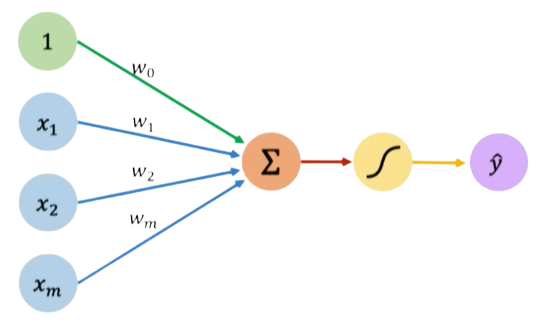
\includegraphics[width=\textwidth]{graphics/nobg perceptron.png}
    \end{center}
    \caption{Schematic diagram of a perceptron,\textit{Src: MIT Introduction to Deep Learning,6.S191,Lec-1}}\label{perceptron}
\end{marginfigure} 
We assume the perceptron returns a high value when it detects $P$. The inputs to a perceptron can be features from known observation or outputs of other neuron. Let the inputs be $x_1,x_2\hdots x_n$. We arrange them neatly in a vector $X=[x_1,x_2,x_3\hdots x_n]$. Each of those $x_i$s can be thought to be the presence and absence of a simpler feature. We take a weighted sum of those inputs to get $s=\sum_{1\leq i\leq n}w_ix_i+w_0$. The intuition is the magnitude of $w_i$ is a measure of the importance of feature $x_i$ and the sign is the direction in which $x_i$ affects the feature which the perceptron is detecting. For example, if the perceptron is detecting if the input is 8 and $x_i$ is the output from another perceptron that detects if a straight line is present then $w_i$ will be negative: there is no straight line in 8. On the other hand,  $x_j$ is the output from another perceptron that detects if a circle is present then $w_i$ will be positive: there are two of them in 8. $w_0$ is just a centering constant. The output of the perceptron will be $y=\sigma(s)$, where $\sigma$ is known as the activation function. 
\chapter{How to train a neural network}
\section{Introduction}
Once we have made our model of a neural network, we would like to train it. The process of training involves tuning the set of weights $W=[w_0,w_1,w_2\hdots]$ associated with each perceptron. To do so we shall give the neural network a rigorous mathematical structure and look at methods to efficiently adjust our weights.
\section{The loss functions}
\begin{marginfigure}
    \begin{center}
        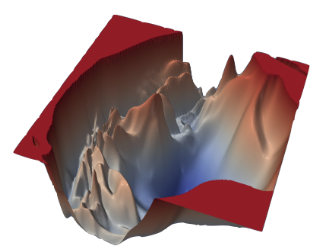
\includegraphics[width=\textwidth]{graphics/resnet110-noskip-loss.png}
    \end{center}
    \caption{A slice of the loss landscape(A graph of $\mathcal L$ vs $(w_i,w_j)$) in ResNet(an example of a type of neural network). Note that it is quite hard to find the minima in this.\citep{li2018visualizing}}
\end{marginfigure}
The loss function can be thought to be a measure of the efficiency of a neural network. Suppose we have a set of observations $ X_0=[X_1,X_2,\hdots X_n]$ with known labels/values $Y_0=[Y_1,Y_2\hdots Y_n]$. Assume our neural network gives predictions $\hat Y_0=[\hat Y_1,\hat Y_2\hdots Y_n]$. Then loss function $\mathcal L(\hat Y_i,Y_i)$ calculates how off our prediction was from the actual label. We define the total loss as $\mathcal L(\hat Y_0,Y_0)=\sum\mathcal L(\hat Y_i,Y_i)$. Generally, we use mean square error(MSE) as the loss function for regression problems and categorical cross entropy for classification problems. That being said, in more complex network, the loss function may be more complicated. For example, a common problem in computer vision is to identify objects in an image. It is found that it is easier to answer the question in two parts:
\begin{enumerate}
    \item Is there an object present in the image?
    \item If yes, where is it in the image?
\end{enumerate}

As we can understand, the first question is a classification problem whereas the second question is a regression problem(assuming we give our answer as coordinates). Now that we have a measure of how good our neural network is, we can think of training to be tuning the parameters to minimise loss.
\section{Gradient Descent}
\begin{marginfigure}
    \begin{center}
        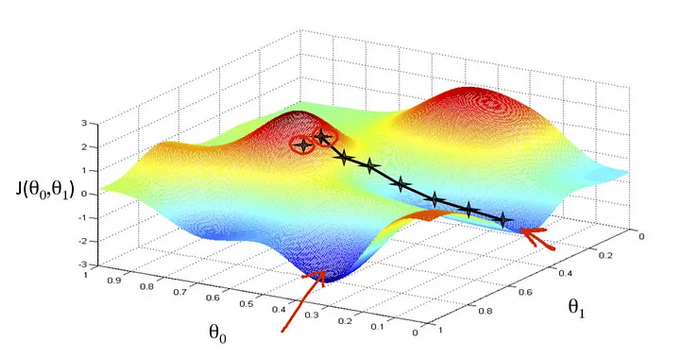
\includegraphics[width=\textwidth]{graphics/grad-desc.png}
    \end{center}
    \caption{Gradient descent, Src: https://towardsdatascience.com/an-intuitive-explanation-
    of-gradient-descent-83adf68c9c33}
\end{marginfigure}
To find the correct set of weights, we use a greedy approach. We check the surrounding landscape
of the weight(i.e. calculate the gradient) and take a step in the direction which leads to maximum
decrease in L. This is an iterative process. Mathematically, for the weight $w_i$ we have the following
update rule:
$$w_i\to w_i-\eta\frac{\partial \mathcal L}{\partial w_i}$$
$\eta$ is known as the learning rate. Fixing $\eta$ is quite tricky: too large and it shoots part the minima, too small and it never converges. The best way to do it is to  use an adaptive learn rate. Some methods(parametric, non-parametric and
hybrid are discussed later, once we cover back propagation)

\section{Neural network as a directed acyclic graph (DAG)}
We look at neural network as a DGA. Each variable (output of perceptron, weight and feature of input) is a vertex. An edge connects vertex $v_i$ to $v_j$ if $v_i$ is directly needed for the computation or updation of $v_j$. For a perceptron with output $x=\sigma\left(w_0+\sum w_ix_i\right)$, there are edges from all $x_i$ and $w_i$ to $x$. In some cases, $\eta$ is not a constant. In that case, there are edges from the parameters $\eta$ depend on to $x$.

\section{Reverse mode auto differentiation}
The general algorithm that is used for gradient descent is called backpropagation. In it's most basic implementation the running time is exponential in the number of layers, which is undesirable. So we talk about a slightly different implementation known as reverse mode auto differentiation$^*$\marginnote{$^*$As it turns out, people in control theory were using this way before this was independently invented for use in deep learning. Kinda shows how low inter topic information sharing is}. Each iteration takes place in two steps: the forward phase and the backward phase. 
\subsection{Forward phase}
In the forward phase, the algorithm simply calculates the total loss $\mathcal L(\hat Y_0,Y_0)$. This is called the forward phase as we calculate along the direction of the edge. 
\subsection{Backward phase}
In that backward phase we calculate the gradients and update weights. We calculate the gradients by repeatedly applying chain rule. If there is an edge from $v_i$ to $v_j$ then $\frac{\partial v_j}{\partial v_i}$ can be calculated directly.  If they don't have an edge connecting them, we take the product of the derivatives  along the edges on a path and then take the sum along all the paths. A small example is given in \ref{chainRule}
\begin{marginfigure}
    \begin{center}
        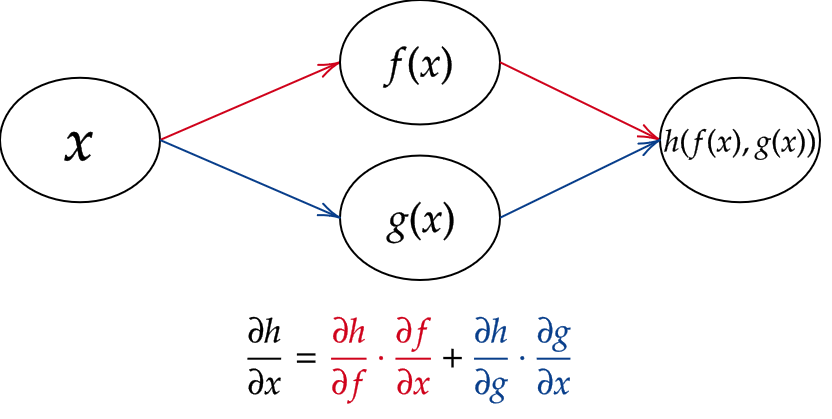
\includegraphics[width=\textwidth]{graphics/chain.png}
    \end{center}
    \caption{A small example of chain rule application}\label{chainRule}
\end{marginfigure}  
At this point it should be obvious that this process is going to take exponentially long the deeper the network is: there are simply too many paths. Here we use dynamic programming. Consider the example in \ref{path}

We see that certain terms are repeated in the expression. This is because parts of the path(shown in colored arrows) is repeated. Therefore, if we can store the gradients for some edges then we don't need to calculate all the terms every time. This significantly reduces computation and makes the algorithm practical to implement. This is called the backward phase as the gradients are calculated against the direction of the edges. 
\section{Gradient Descent Strategies}
\subsection{Stochastic Gradient Descent}
\begin{marginfigure}
    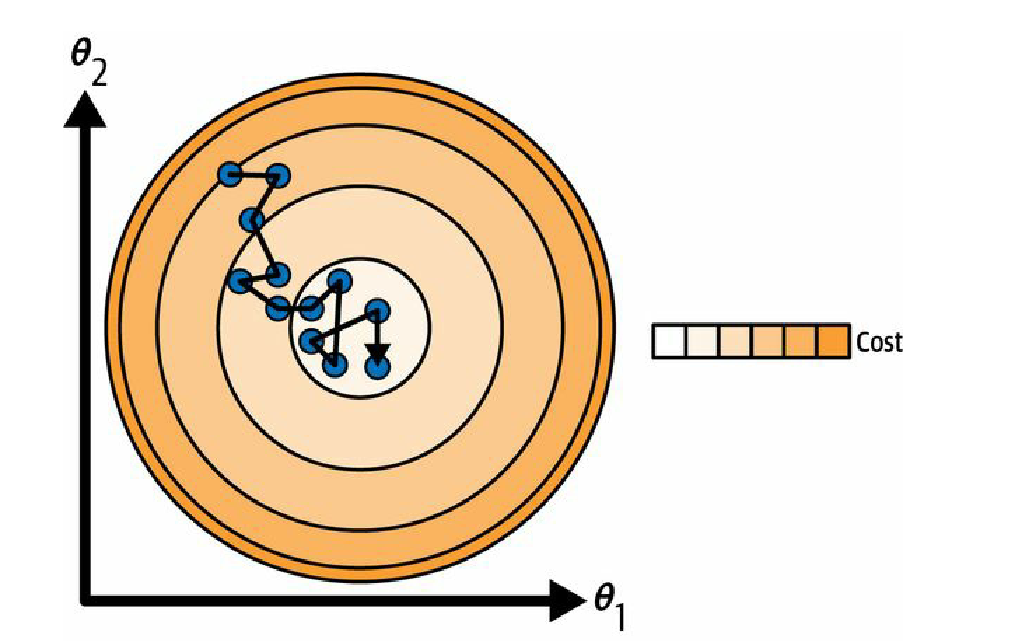
\includegraphics[width=\textwidth]{graphics/stochastic gradient descent.png}
    \caption{Stochastic Gradient Descent. Note that we don't take steps on the best direction, but it is faster.\citep{geron2022hands}}
\end{marginfigure}
Instead of calculating the total loss, we calculate the loss from a randomly picked sample(or a
batch in case of batch gradient descent). Since we are no longer calculating the total loss over all
data points, this decreases the computational time. A proper analogy might be instead of taking
slower but confident steps, we take faster but less-confident steps.
\subsection{Normalization}
\begin{marginfigure}
    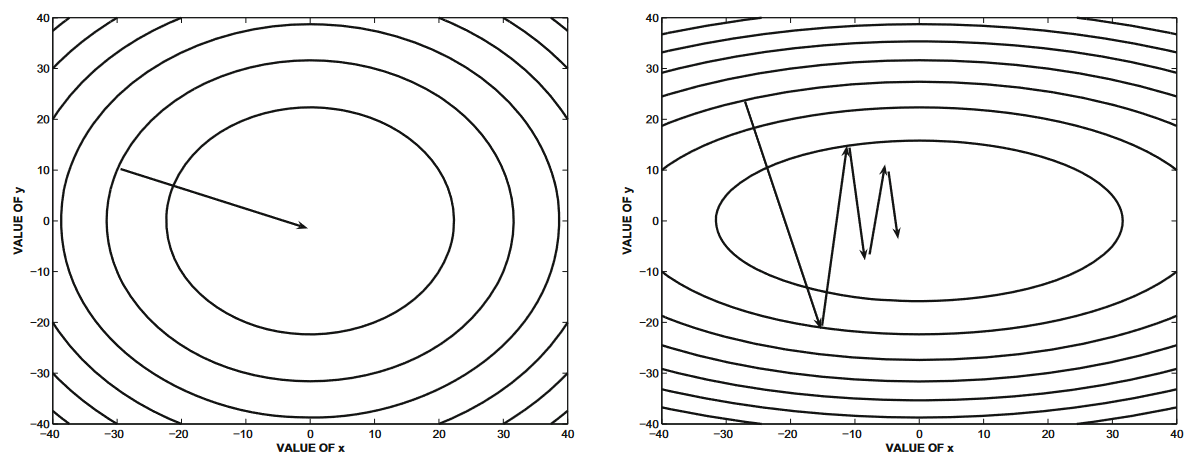
\includegraphics[width=\textwidth]{graphics/normalise.png}
    \caption{Normalization\citep{aggarwal2018neural}}
\end{marginfigure}
Normalizing features is a way to make the descent smoother. It essentially lowers gradient in
directions orthogonal to the minima. This also eases setting the learning rate. If one feature varies between $0$ to 255 and other between 0 and 1, it can be very difficult to set a base learning rate. Normalizing features solves this problem.  
\subsection{Momentum}
\begin{marginfigure}
    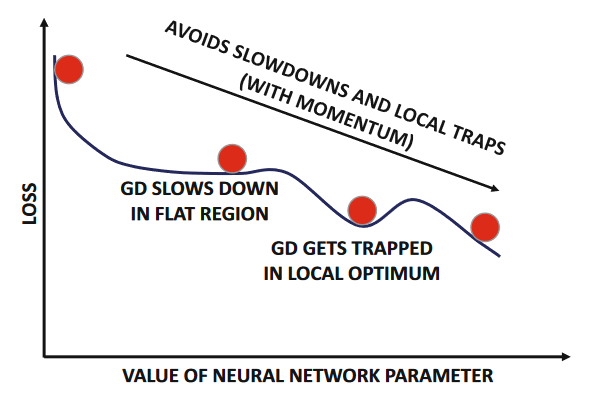
\includegraphics[width=\textwidth]{graphics/momentum.png}
    \caption{Momentum preventing getting stuck at local minima\citep{aggarwal2018neural}}
\end{marginfigure}\begin{marginfigure}
    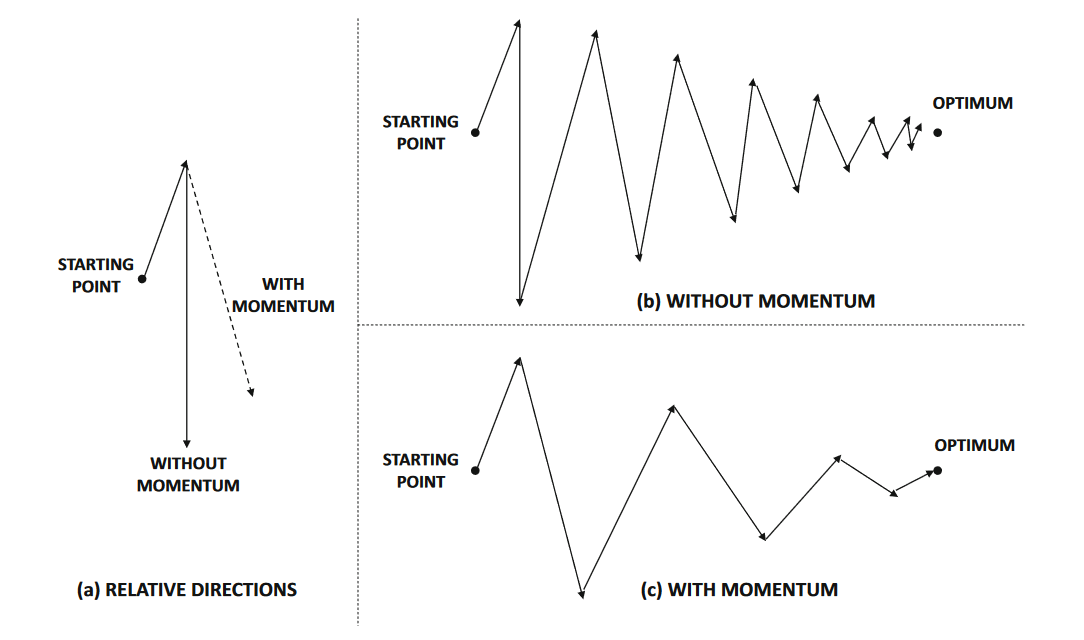
\includegraphics[width=\textwidth]{graphics/momentum-zigzag.png}
    \caption{Momentum reducing zig-zag\citep{aggarwal2018neural}}
\end{marginfigure}
A Momentum term might be used in gradient descent where consideration is made for a moving
average "velocity"  of the descent. Such strategies are particularly helps when there are local
minimas and flat regions. Also helps when there is a lot of ”zig-zag” but the descent on an
average heads in a certain direction. We can improve on this by doing some scout ahead. This
is known as Nestov momentum, and it helps as knowing what's coming up ahead further helps
in correcting the direction of descent.
\begin{figure*}
    \begin{center}
        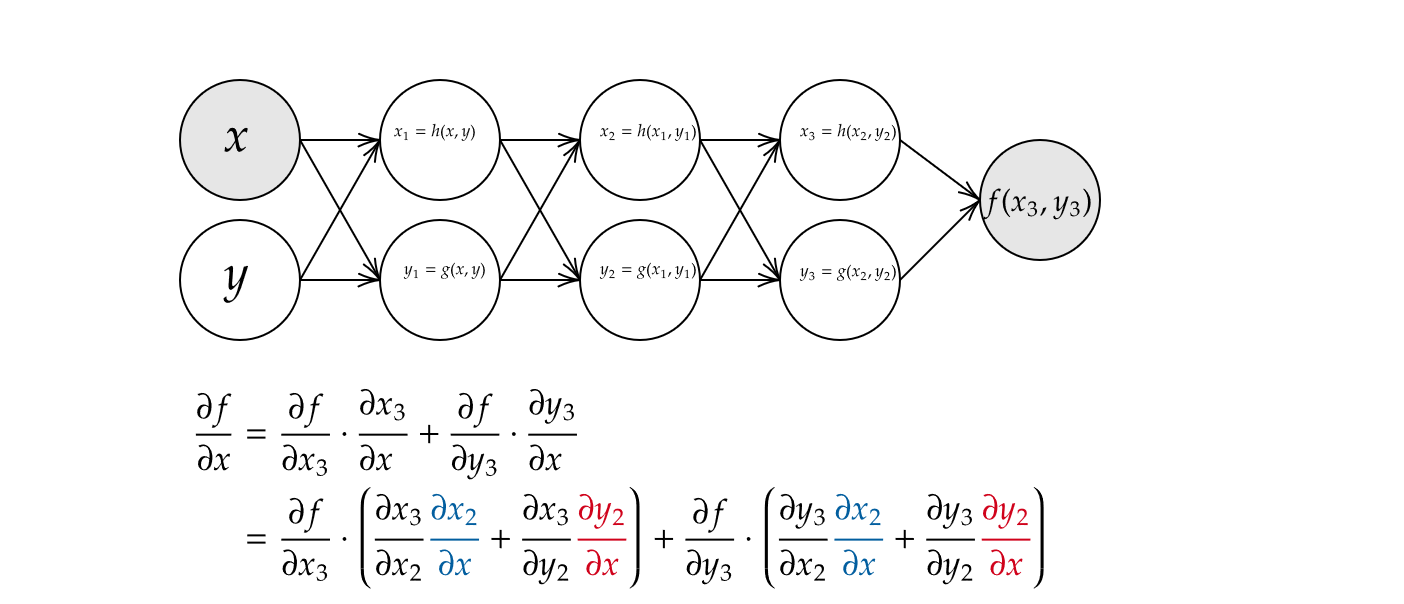
\includegraphics[width=\textwidth]{graphics/revmodeautodiff.png}
        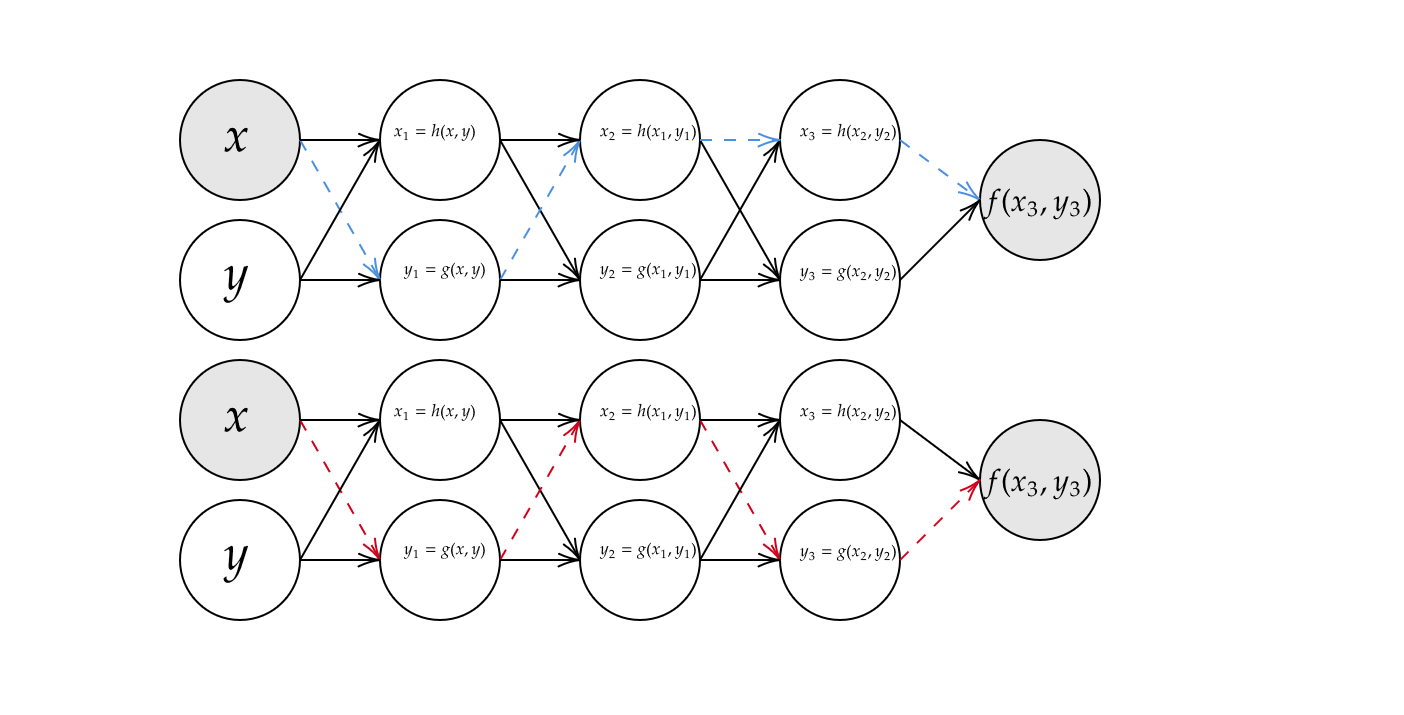
\includegraphics[width=\textwidth]{graphics/path comp.png}
    \end{center}
    \caption{Chain rule in deep networks}\label{path}
\end{figure*}
\section{Setting the learning rate}
\begin{figure}
    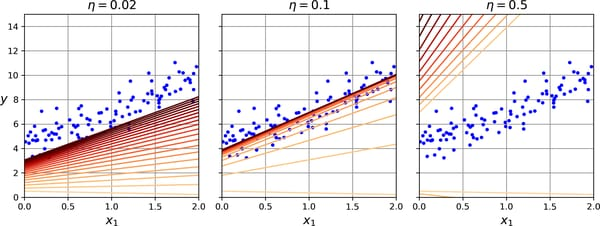
\includegraphics[width=\textwidth]{graphics/learning rate.jpeg}
    \caption{Why is setting a proper learning rate important\citep{geron2022hands}}
\end{figure}
\subsection{Adaptive learning rate}
One way to take care of this problem is  to let different parameters have different learning rates. The idea is that parameters with large partial derivatives are often oscillating
and zigzagging, whereas parameters with small partial derivatives tend to be
more consistent but move in the same direction.
Algorithms include AdaGrad, RMSProp and AdaDelta. Parametric algorithms
combined with momentum considerations also exist: RMSProp with Nesterov
Momentum, ADAM and it's variants like AdaMax, Nadam and AdamW. A quick
comparison table is available at \citep{geron2022hands}
\subsection{Learning rate scheduling}
We have the learning rate high at first so
that it gets a relative idea about where the
minima lies, and then we lower it to find it
with more accuracy. Scheduling is done on numbers of iterations
completed(each iteration is also called an
epoch)
\begin{marginfigure}
    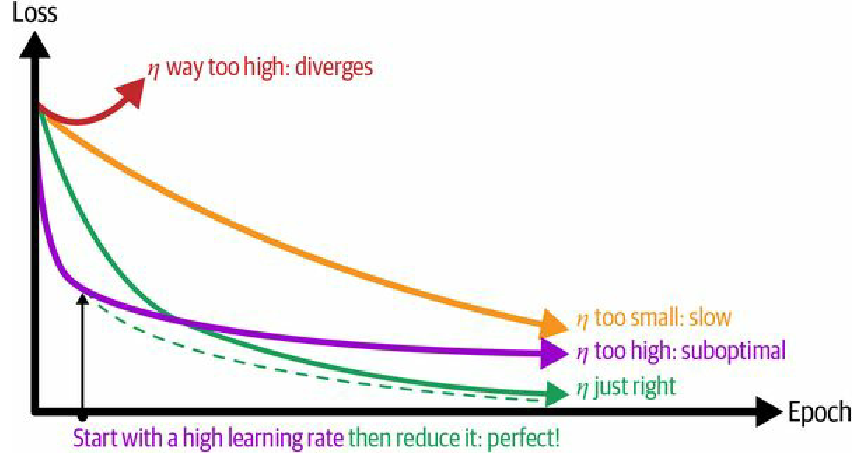
\includegraphics[width=1.3\textwidth]{graphics/learning rate schedule.png}\caption{Learning rate scheduling\citep{geron2022hands}}
\end{marginfigure}
\subsection{One cycle scheduling}
The basic idea behind one cycle scheduling is to start with a low learning
rate, gradually increase it to a maximum value, and then decrease it again to
a low value. This approach helps the network explore a wide range of
learning rates, allowing it to quickly converge to a good solution and
potentially escape from local minima. By using a cyclical learning rate schedule, one cycle scheduling aims to strike
a balance between exploration and exploitation in the learning process. It
enables the network to quickly explore a wide range of learning rates at the
beginning and then gradually refine its weights as the learning rate
decreases.
\section{Choosing Activation function}
The loss function and the gradients propagated backwards depend on the activation functions used. A bad activation function(for example, a function which is not differentiable everywhere) can make training very hard. We first look at some 

\part{Deep Learning in NLP}

\chapter{Why is language a pain to model? And how do we model them.}
\section{Language and ideas}
Language arose about $100,000-1,000,000$ years ago and that took us from Bronze Age to modern science. From a linguistic point of view, a word is the representation of an idea. Words representing old obsolete ideas are often forgotten, and new words representing new ideas. 


\section{Why is NLP hard?}
\textit{Written as a person fluent in English, Bengali and Hindi}\\
The short answer is when we speak, we leave out massive chunks of information. A lot of the information  conveyed while writing assumes that the reader has prior context and experience to extract meaningful information from the text. It is even more difficult when looking at transcriptions of spoken text: While speaking we use our facial expressions and vocal tones as a part of communication.  Some particular difficulties are described below:
\begin{enumerate}
    \item Homonyms: When we say "He/She is cool" we often mean that a person is calm and collected. We use our prior experience to infer "cool" is not referring to feeling coldness. Ideally, we would like our model to understand such subtleties. More examples include:
    \begin{itemize}
        \item \textbf{Iraqi Head Seeks Arms}: Here head is to be interpreted as leader and not as body part. 
        \item \textbf{Kids Make Nutritious Snacks}: Here make is to be understood as the process of creation and is not meant as a part of. 
        \item \textbf{Miners Refuse to Work after Death}: Here death refers to death of a person and not the state of being dead.
    \end{itemize}
    \item For complex sentences we use prior experiences for deciphering meaning. This process is made more complex by the fact that in English language, a single word can act as different parts of speech. For example, 
    \begin{itemize}
        \item \textbf{Enraged Cow Injures Farmer with Ax}: the with ax part is describing the farmer and not the cow.
        \item \textbf{Hospitals are Sued by 7 Foot Doctors}: The phrase"7 foot" are two different ideas: 7 describes the number of doctors and foot describes their specialty of work. 
        \item \textbf{Students cook and serve grandparents}: Grandparents are served food, they are not the food
    \end{itemize}
    More examples are available here:\\
    \verb|https://www.plainlanguage.gov/resources/humor/funny-headlines/|
    \item Figures of speech: We use the example of sarcasm. When we use sarcasm we mean the opposite of what we say. We again use prior experience to identify that the writer doesn't mean what they say. For example, consider a very simple case: "Great! Now my tires are flat". We use our prior knowledge that a flat tire (in most cases) is not a desirable thing and so the word "great" is not used in a positive sense. Things get tricker when this is used in more subtle sense.
    \item Not all ideas are available in all languages: As a very artificial example, no $16^{th}$ century Indian language would have a word for potato simply because no one knew what a potato was! Some more examples are available here:\\ \verb|https://www.babbel.com/en/magazine/untranslatable-01|
    \item As someone once said, language is a living thing. New words are always being made to represent new ideas and the internet has accelerated this process. Words like Poggers, KEKW, OC etc. were invented in the era of memes and twitch chat. Usage of unalive (which was not an actual word some time ago) is gaining popularly as the actual word "dead" is often flagged by online platforms. 
\end{enumerate}




\section{Context and Lexical semantics}
Each word represents an idea, and when we communicate we chain those ideas. This gives rise to the idea of context. We claim a word gets it's meaning from the words surrounding it. For example, if we have a new word \textbf{plompyskompy} and we say it is used as follows: "There is an apple \textbf{plompyskompy} on the table" you might (again, due to your experience) understand it represents same kind of idea the word "on"  represents. You understand this due to the words surrounding it.  This leads us to the idea of Lexical semantics(Ref: \verb|https://en.wikipedia.org/wiki/Lexical_semantics|)



\section{Language as a Markov process}
This will now be a quick discussion. A word gets it's meaning from its surrounding words. The rest of the corpus doesn't matter. What came 100 words ago doesn't matter(unless we are considering what came 100 words ago to be a part of the context of the word). We look at the last few words and by our theory, it should be enough to predict what our next word is going to be. Therefore, if we are looking at a context window of $n$ words then it should be modelled as an $n^{th}$ order Markov chain. Ref:\\\verb|https://www.cs.princeton.edu/courses/archive/spr05/cos126/assignments/markov.html|

\section{Language as a stochastic process}
Languages can also be modelled as stochastic process, i.e. we drop the assumption that local context is all that is needed. And it should be noted that the memoryless property of Markov processes are counterintuitive to our claim that experience plays an important role in decoding ideas from sentences. Ref: \verb|https://openreview.net/forum?id=pMQwKL1yctf|

\section{Crude early models and their shortcomings}

 Traditionally, a computer understands a word by using a dictionary and looking up synonyms(word with similar meaning), hypernyms(expression of belonging to a more general category), hyponyms(expression of belonging to more specific subclass). A minimal example implemented in NLTK is shown below. Some arrays are truncated for brevity.
    \begin{lstlisting}
        >>> from nltk.corpus import wordnet as wn
        >>> wn.synonyms('car')
        [['auto', 'automobile', 'machine', 'motorcar'], ['railcar', 'railroad_car', 'railway_car'], ['gondola'], ['elevator_car'], ['cable_car']]
        >>> wn.synsets('car')[:2]
        [Synset('car.n.01'), Synset('car.n.02')]
        >>> wn.synset('car.n.01').definition()
        'a motor vehicle with four wheels; usually propelled by an internal combustion engine'
        >>> wn.synset('car.n.01').examples()
        ['he needs a car to get to work']
        >>> wn.synset('car.n.01').hypernyms()
        [Synset('motor_vehicle.n.01')]
        >>> wn.synset('dog.n.01').hypernyms()    
        [Synset('canine.n.02'), Synset('domestic_animal.n.01')]
        >>> wn.synset('car.n.01').hyponyms()[:5]
        [Synset('ambulance.n.01'), Synset('beach_wagon.n.01'), Synset('bus.n.04'), Synset('cab.n.03'), Synset('compact.n.03')]
    \end{lstlisting}
But this is not a very robust solution: dependency on context and nuances are not resolved(Ex: "crimson" is a synonym of "red" but "the color of an apple is crimson" is a weird sounding sentence).  Moreover, language is ever-changing and keeping track of an ever changing 
    \begin{marginfigure}%
        
    \end{marginfigure}%
In traditional bag of words approach, words are given a one hot vector representation. For example:
\begin{align*}
    \text{"hotel"}=[0,0,0,0,0,1,0,0,0]\\
    \text{"motel"}=[0,0,0,0,0,0,0,1,0]
\end{align*}
But this approach has its own limitations:
\begin{enumerate}
    \item Vector size increase with increase in vocabulary
    \item We understand that the words above are similar, but that similarity is not reflected in such one-hot encoding.
\end{enumerate}






\chapter{Word Embeddings}

\section{Why vectors?}
We would like to have a structure 
\begin{enumerate}
    \item that can be modelled using a small(<- this depends on what your idea of small is, but we would like to have a memory efficient approach) number of parameters
    \item that has an inbuilt idea of similarity
    \item that can be easily manipulated
\end{enumerate}
As it turns out finite dimensional vector spaces are perfect for this task: the number of parameters is the number of dimensions, a metric can be used as notion of similarity, and we already have tools to manipulate them.





\section{Data Preparation}
We need to prepare the data or the next two models. We select a window size $n$. From the corpus, $n$ consecutive words are sampled. The middle word is the target word and the rest is the context. Each such target word, context pair is a data point.



\section{One-hot Representation of Words and Context}

Once the data preparation is done we will have a set of data points of the form $(S,W)$ where $S$ is the context and $W$ is the word. If the word is in the $i^{th}$ place in the vocabulary $V$ then we represent $W$ the one-hot vector $e_i$ ($i^{th}$ element of the standard basis). If the context contains the words $W_1=V[\alpha_1], W_2=V[\alpha_2]\hdots W_n=V[\alpha_n]$ then we will represent the context $S$ as $\sum_{i=1}^ne_{\alpha_i}$, i.e. the sum of the one-hot encoding of the individual words. For the rest of this discussion I will use the notation $w_i,V[i]$ and $e_i$ interchangeably for words. 








\section{Continuous bag of words model(CBOW)}
Assume we have a data point(we have taken size 5 for the example, but this should be adjusted as needed) as follows:
\begin{center}
    \textcolor{red}{Word1 Word 2} Word \textcolor{red}{Word3 Word 4}
\end{center} 
We model a classification problem where given context $\{$Word1, Word2, Word3, Word4$\}$ we wish to classify which word this set provides context for.[Note, when we represent it as a set, we automatically let go the notion of a sequence- hence the name 'bag of words']. For this we shall use a feed forward network described below:
\begin{enumerate}
    \item \textbf{Input :}For context $S\subset V$, we make an input vector $v$ where:
    $$v_S=\sum_{w_i\in S}e_i$$
    \item  \textbf{Hidden Layer 1}: This is obtained by multiplying $v$ by a matrix $W$. We denote:
    $$h_S=Wv_S$$
    For a single word $w_i$, $h_i=We_i=i^{th}$ column of $W$ will represent the hidden representation of $w_i$. 
    Therefore, if our context contains is $S=\{w_{\alpha_1},w_{\alpha_2},w_{\alpha_3},w_{\alpha_4}\hdots w_{\alpha_n}\}$ then our hidden representation of the context will be $h_S=W\left(\sum_{k=1}^n e_{\alpha_k}\right)=\sum_{k=1}^n h_{w_{\alpha_k}}$ (Note how our choice of using a linear space as structure of choice and setting the context as the linear combination of its constituents comes handy here)
    \item \textbf{Hidden Layer 2}: We use another matrix $W'$ and get
    $$y=W'h_S$$
    \item \textbf{Hidden Layer 3}: This is just a soft max to normalize things:
    $$\hat y=\text{Softmax}(y)$$
\end{enumerate} 
We use cross-entropy as our loss function of choice to train the model. $\hat y$ is compared to the one-hot representation of the word.

\begin{figure}
    \begin{center}
        

\tikzset{every picture/.style={line width=0.75pt}} %set default line width to 0.75pt        

\begin{tikzpicture}[x=0.75pt,y=0.75pt,yscale=-1,xscale=1]
%uncomment if require: \path (0,744); %set diagram left start at 0, and has height of 744

%Shape: Rectangle [id:dp026521693413700476] 
\draw   (172,20) -- (182,20) -- (182,210) -- (172,210) -- cycle ;
%Straight Lines [id:da6320135821235765] 
\draw    (192,110) -- (250,110) ;
\draw [shift={(252,110)}, rotate = 180] [color={rgb, 255:red, 0; green, 0; blue, 0 }  ][line width=0.75]    (10.93,-3.29) .. controls (6.95,-1.4) and (3.31,-0.3) .. (0,0) .. controls (3.31,0.3) and (6.95,1.4) .. (10.93,3.29)   ;
%Shape: Rectangle [id:dp12692840020505802] 
\draw   (262,70) -- (272,70) -- (272,150) -- (262,150) -- cycle ;
%Straight Lines [id:da7459277485193251] 
\draw    (282,110) -- (340,110) ;
\draw [shift={(342,110)}, rotate = 180] [color={rgb, 255:red, 0; green, 0; blue, 0 }  ][line width=0.75]    (10.93,-3.29) .. controls (6.95,-1.4) and (3.31,-0.3) .. (0,0) .. controls (3.31,0.3) and (6.95,1.4) .. (10.93,3.29)   ;
%Shape: Rectangle [id:dp07310081517407963] 
\draw   (352,20) -- (362,20) -- (362,210) -- (352,210) -- cycle ;
%Straight Lines [id:da06986407926721172] 
\draw    (372,110) -- (430,110) ;
\draw [shift={(432,110)}, rotate = 180] [color={rgb, 255:red, 0; green, 0; blue, 0 }  ][line width=0.75]    (10.93,-3.29) .. controls (6.95,-1.4) and (3.31,-0.3) .. (0,0) .. controls (3.31,0.3) and (6.95,1.4) .. (10.93,3.29)   ;
%Shape: Rectangle [id:dp04257972028230528] 
\draw   (452,20) -- (462,20) -- (462,210) -- (452,210) -- cycle ;
%Shape: Rectangle [id:dp9098181133670411] 
\draw   (120,290) -- (130,290) -- (130,400) -- (120,400) -- cycle ;
%Straight Lines [id:da16252267787659302] 
\draw    (132,340) -- (190,340) ;
\draw [shift={(192,340)}, rotate = 180] [color={rgb, 255:red, 0; green, 0; blue, 0 }  ][line width=0.75]    (10.93,-3.29) .. controls (6.95,-1.4) and (3.31,-0.3) .. (0,0) .. controls (3.31,0.3) and (6.95,1.4) .. (10.93,3.29)   ;
%Shape: Rectangle [id:dp7664434843570327] 
\draw   (202,310) -- (210,310) -- (210,370) -- (202,370) -- cycle ;
%Straight Lines [id:da575597764045124] 
\draw    (340,470) -- (398,470) ;
\draw [shift={(400,470)}, rotate = 180] [color={rgb, 255:red, 0; green, 0; blue, 0 }  ][line width=0.75]    (10.93,-3.29) .. controls (6.95,-1.4) and (3.31,-0.3) .. (0,0) .. controls (3.31,0.3) and (6.95,1.4) .. (10.93,3.29)   ;
%Shape: Rectangle [id:dp7323495271401276] 
\draw   (410,380) -- (420,380) -- (420,570) -- (410,570) -- cycle ;
%Straight Lines [id:da16269082378611044] 
\draw    (430,470) -- (488,470) ;
\draw [shift={(490,470)}, rotate = 180] [color={rgb, 255:red, 0; green, 0; blue, 0 }  ][line width=0.75]    (10.93,-3.29) .. controls (6.95,-1.4) and (3.31,-0.3) .. (0,0) .. controls (3.31,0.3) and (6.95,1.4) .. (10.93,3.29)   ;
%Shape: Rectangle [id:dp33808841681535384] 
\draw   (510,380) -- (520,380) -- (520,570) -- (510,570) -- cycle ;
%Shape: Rectangle [id:dp7307300567221867] 
\draw   (120,420) -- (130,420) -- (130,530) -- (120,530) -- cycle ;
%Straight Lines [id:da39746393944318226] 
\draw    (132,470) -- (190,470) ;
\draw [shift={(192,470)}, rotate = 180] [color={rgb, 255:red, 0; green, 0; blue, 0 }  ][line width=0.75]    (10.93,-3.29) .. controls (6.95,-1.4) and (3.31,-0.3) .. (0,0) .. controls (3.31,0.3) and (6.95,1.4) .. (10.93,3.29)   ;
%Shape: Rectangle [id:dp6685146380753737] 
\draw   (202,440) -- (210,440) -- (210,500) -- (202,500) -- cycle ;
%Shape: Rectangle [id:dp40808635862127074] 
\draw   (120,550) -- (130,550) -- (130,660) -- (120,660) -- cycle ;
%Straight Lines [id:da5587676126883278] 
\draw    (132,600) -- (190,600) ;
\draw [shift={(192,600)}, rotate = 180] [color={rgb, 255:red, 0; green, 0; blue, 0 }  ][line width=0.75]    (10.93,-3.29) .. controls (6.95,-1.4) and (3.31,-0.3) .. (0,0) .. controls (3.31,0.3) and (6.95,1.4) .. (10.93,3.29)   ;
%Shape: Rectangle [id:dp6700192839775068] 
\draw   (202,570) -- (210,570) -- (210,630) -- (202,630) -- cycle ;
%Shape: Rectangle [id:dp8434692403820858] 
\draw   (320,440) -- (330,440) -- (330,500) -- (320,500) -- cycle ;
%Straight Lines [id:da7635704939549399] 
\draw    (220,340) -- (308.86,468.36) ;
\draw [shift={(310,470)}, rotate = 235.3] [color={rgb, 255:red, 0; green, 0; blue, 0 }  ][line width=0.75]    (10.93,-3.29) .. controls (6.95,-1.4) and (3.31,-0.3) .. (0,0) .. controls (3.31,0.3) and (6.95,1.4) .. (10.93,3.29)   ;
%Straight Lines [id:da1717667506724866] 
\draw    (220,600) -- (308.86,471.64) ;
\draw [shift={(310,470)}, rotate = 124.7] [color={rgb, 255:red, 0; green, 0; blue, 0 }  ][line width=0.75]    (10.93,-3.29) .. controls (6.95,-1.4) and (3.31,-0.3) .. (0,0) .. controls (3.31,0.3) and (6.95,1.4) .. (10.93,3.29)   ;
%Straight Lines [id:da6154675184222768] 
\draw    (220,470) -- (308,470) ;
\draw [shift={(310,470)}, rotate = 180] [color={rgb, 255:red, 0; green, 0; blue, 0 }  ][line width=0.75]    (10.93,-3.29) .. controls (6.95,-1.4) and (3.31,-0.3) .. (0,0) .. controls (3.31,0.3) and (6.95,1.4) .. (10.93,3.29)   ;

% Text Node
\draw (213,92.4) node [anchor=north west][inner sep=0.75pt]    {$W$};
% Text Node
\draw (303,92.4) node [anchor=north west][inner sep=0.75pt]    {$W'$};
% Text Node
\draw (374,92.4) node [anchor=north west][inner sep=0.75pt]  [font=\small]  {$Softmax$};
% Text Node
\draw (144,212.4) node [anchor=north west][inner sep=0.75pt]    {$Context$};
% Text Node
\draw (217,152.4) node [anchor=north west][inner sep=0.75pt]    {$ \begin{array}{l}
\ \ \ \ \ \ Hidden\\
Representation\\
\ \ \ of\ Context
\end{array}$};
% Text Node
\draw (350,212.4) node [anchor=north west][inner sep=0.75pt]    {$y$};
% Text Node
\draw (454,212.4) node [anchor=north west][inner sep=0.75pt]    {$\hat y$};
% Text Node
\draw (321,252.4) node [anchor=north west][inner sep=0.75pt]    {$( a)$};
% Text Node
\draw (153,322.4) node [anchor=north west][inner sep=0.75pt]    {$W$};
% Text Node
\draw (361,452.4) node [anchor=north west][inner sep=0.75pt]    {$W'$};
% Text Node
\draw (432,452.4) node [anchor=north west][inner sep=0.75pt]  [font=\small]  {$Softmax$};
% Text Node
\draw (408,572.4) node [anchor=north west][inner sep=0.75pt]    {$y$};
% Text Node
\draw (512,572.4) node [anchor=north west][inner sep=0.75pt]    {$\hat y$};
% Text Node
\draw (71,332.4) node [anchor=north west][inner sep=0.75pt]    {$Word$};
% Text Node
\draw (153,452.4) node [anchor=north west][inner sep=0.75pt]    {$W$};
% Text Node
\draw (71,462.4) node [anchor=north west][inner sep=0.75pt]    {$Word$};
% Text Node
\draw (153,582.4) node [anchor=north west][inner sep=0.75pt]    {$W$};
% Text Node
\draw (71,592.4) node [anchor=north west][inner sep=0.75pt]    {$Word$};
% Text Node
\draw (245,452.4) node [anchor=north west][inner sep=0.75pt]    {$Sum$};
% Text Node
\draw (271,502.4) node [anchor=north west][inner sep=0.75pt]    {$ \begin{array}{l}
\ \ \ \ \ \ Hidden\\
Representation\\
\ \ \ of\ Context
\end{array}$};
% Text Node
\draw (318,662.4) node [anchor=north west][inner sep=0.75pt]    {$( b)$};
% Text Node
\draw (154,631.4) node [anchor=north west][inner sep=0.75pt]    {$ \begin{array}{l}
\ \ \ \ \ \ Hidden\\
Representation\\
\ \ \ of\ Word
\end{array}$};


\end{tikzpicture}
\caption{Equivalent expression of CBOW}
    \end{center}
\end{figure}
We have:
$$\hat y=Softmax(W'(h_S))$$
But as $h_S$ is independent of all $h_{w}$ where $w\notin S$. Therefore, we don't compute $Wv_s$ nor do we keep track of all the weights. We look only at those columns of $W$ that correspond to words in the context and don't care about the rest. 
\subsection{Interpretation on a two word window}
Assume we have a two word window. We use a data point $(w_\alpha,w_\beta)$. Note that:
$$\mathcal{L}(w_\beta)=-\log \hat y_\beta=-\log\left(\frac{e^{y_\beta}}{\sum_{r} e^{y_r}}\right)$$
We do back propagation and calculate the gradients:
\begin{align*}
    \frac{\partial \mathcal L}{\partial y_i}=\hat y_i-\delta(i,\beta)
\end{align*}
Denote this as $E_i$ and define $E=[E_1, E_2\hdots E_n]$. Note $E=\hat y-$Observed $y$
\begin{align*}
    \frac{\partial \mathcal L}{\partial h_i}=\sum_{j}\frac{\partial \mathcal L}{\partial y_j}\frac{\partial y_j}{\partial h_i}= \sum_j E_j\frac{\partial \sum_k h_k W'_{k,j}}{\partial h_i}=\sum_j E_jW'_{ij}
\end{align*}
Therefore the gradient with respect to $h$ is
$$\nabla \mathcal L=W'^TE$$
This gives the update rules for $h$ as 
$$h:=h-\eta\nabla \mathcal L=h- \eta W\hat y+\eta W\text{ Observed }y$$
Assume  initial entries of $W$ to be small. Then and therefore, entries of $h_{Cat}$ and $h_{Dog}$ will have similar starting values: almost 0. Look at the following sentences:
\begin{center}
    Cat \textcolor{red}{sleeps}\\
    Dog \textcolor{red}{sleeps}
\end{center}
Note in both those cases, Observed $y$ will be same and therefore $h_{cat}$ and $h_{dog}$ will be adjusted in the same direction when they appear in similar context. This idea makes sure that similar words will have similar cosine similarity due to a form of transitive action. 

\section{Skip-Gram}
Skip-gram in a sense is CBOW trained in opposite direction. In this case we use a word to classify what context it comes from. The structure of the model is almost same as before.
\begin{figure}[h]
    \begin{center}
        

\tikzset{every picture/.style={line width=0.75pt}} %set default line width to 0.75pt        

\begin{tikzpicture}[x=0.75pt,y=0.75pt,yscale=-1,xscale=1]
%uncomment if require: \path (0,300); %set diagram left start at 0, and has height of 300

%Shape: Rectangle [id:dp8690317092107768] 
\draw   (192,31) -- (202,31) -- (202,221) -- (192,221) -- cycle ;
%Straight Lines [id:da3129031681625205] 
\draw    (212,121) -- (270,121) ;
\draw [shift={(272,121)}, rotate = 180] [color={rgb, 255:red, 0; green, 0; blue, 0 }  ][line width=0.75]    (10.93,-3.29) .. controls (6.95,-1.4) and (3.31,-0.3) .. (0,0) .. controls (3.31,0.3) and (6.95,1.4) .. (10.93,3.29)   ;
%Shape: Rectangle [id:dp7964817410089358] 
\draw   (282,81) -- (292,81) -- (292,161) -- (282,161) -- cycle ;
%Straight Lines [id:da5578177280290412] 
\draw    (302,121) -- (360,121) ;
\draw [shift={(362,121)}, rotate = 180] [color={rgb, 255:red, 0; green, 0; blue, 0 }  ][line width=0.75]    (10.93,-3.29) .. controls (6.95,-1.4) and (3.31,-0.3) .. (0,0) .. controls (3.31,0.3) and (6.95,1.4) .. (10.93,3.29)   ;
%Shape: Rectangle [id:dp9023443845481357] 
\draw   (372,31) -- (382,31) -- (382,221) -- (372,221) -- cycle ;
%Straight Lines [id:da6062319286919925] 
\draw    (392,121) -- (450,121) ;
\draw [shift={(452,121)}, rotate = 180] [color={rgb, 255:red, 0; green, 0; blue, 0 }  ][line width=0.75]    (10.93,-3.29) .. controls (6.95,-1.4) and (3.31,-0.3) .. (0,0) .. controls (3.31,0.3) and (6.95,1.4) .. (10.93,3.29)   ;
%Shape: Rectangle [id:dp2886304505568057] 
\draw   (472,31) -- (482,31) -- (482,221) -- (472,221) -- cycle ;

% Text Node
\draw (233,103.4) node [anchor=north west][inner sep=0.75pt]    {$W$};
% Text Node
\draw (323,103.4) node [anchor=north west][inner sep=0.75pt]    {$W'$};
% Text Node
\draw (394,103.4) node [anchor=north west][inner sep=0.75pt]  [font=\small]  {$Softmax$};
% Text Node
\draw (164,223.4) node [anchor=north west][inner sep=0.75pt]    {$Word$};
% Text Node
\draw (237,163.4) node [anchor=north west][inner sep=0.75pt]    {$ \begin{array}{l}
\ \ \ \ \ \ Hidden\\
Representation\\
\ \ \ \ \ of\ Word
\end{array}$};
% Text Node
\draw (370,223.4) node [anchor=north west][inner sep=0.75pt]    {$y$};
% Text Node
\draw (474,223.4) node [anchor=north west][inner sep=0.75pt]    {$\hat{y}$};


\end{tikzpicture}

\caption{Schematic diagram of Skip gram}
    \end{center}
\end{figure}
\begin{enumerate}
    \item \textbf{Input :}For word $w_i$, the input is $v=e_i$
    \item  \textbf{Hidden Layer 1}: This is obtained by multiplying $v$ by a matrix $W$. We denote:
    $$h=Wv$$
    \item \textbf{Hidden Layer 2}: We use another matrix $W'$ and get
    $$y=W'h$$
    \item \textbf{Hidden Layer 3}: This is just a soft max to normalize things:
    $$\hat y=\text{Softmax}(y)$$
\end{enumerate}
The target output is  the one-hot representation of the context.
If we have a window size of $n$ our loss function, cross-entropy is the sum of $n-1$ terms. For example, if the data point has context $w_\alpha,w_\beta,w_\gamma,w_\delta$ then the loss function will be:
$$\mathcal L=- \log \hat y_\alpha- \log \hat y_\beta- \log \hat \hat y_\gamma- \log \hat y_\delta$$
Note that gradients are summed. For each term, the update to $h$ is the same as the one for CBOW. We again note that only the $i^{th}$ column of $W$ is updated: therefore we need not keep track of the rest of the weights. The interpretation of CBOW is carried over, this time with multi-word windows. For the sentences:
\begin{center}
    \textcolor{red}{My pet} Cat \textcolor{red}{sleeps}\\
    \textcolor{red}{My pet} Dog \textcolor{red}{sleeps}
\end{center}
Since both gives the same Observed $y$, $h_{Cat}$ and $h_{Dog}$ are adjusted in same direction, making them similar. 

\section{Negative sampling}
To improve performance, we might further want to make sure that words which are not similar are further apart. This gives rise to the idea of negative sampling. We make randomized context-word pairs which don't occur in the corpus. Therefore, we have two sets: $D=\{(S,W)\in Corpus\},D'=\{(S,W)\notin Corpus\}$. Define a random variable $Z$ as:
$$Z=\sigma\left(\hat y_{S}^T\cdot W\right)\text{ or }\sigma\left({S}^T\cdot \hat y_{W}\right)$$
We would like to maximize:
$$P(Z=1|(S,W)\in D)$$
$$P(Z=0|(S,W)\in D')$$
We use now compute the log-likelihood function as follows:\\
$\begin{aligned} & \underset{\theta}{\operatorname{maximize}} \prod_{(w, c) \in D} p(z=1 \mid w, c) \prod_{(w, r) \in D^{\prime}} p(z=0 \mid w, r) \\ & =\underset{\theta}{\operatorname{maximize}} \prod_{(w, c) \in D} p(z=1 \mid w, c) \prod_{(w, r) \in D^{\prime}}(1-p(z=1 \mid w, r)) \\ & =\underset{\theta}{\operatorname{maximize}} \sum_{(w, c) \in D} \log p(z=1 \mid w, c) +\sum_{(w, r) \in D^{\prime}} \log (1-p(z=1 \mid w, r)) \\ & =\underset{\theta}{\operatorname{maximize}} \sum_{(w, c) \in D} \log \frac{1}{1+e^{-v_c^T v_w}}+\sum_{(w, r) \in D^{\prime}} \log \frac{1}{1+e^{v_r^T v_w}} \\ & =\underset{\theta}{\operatorname{maximize}} \sum_{(w, c) \in D} \log \sigma\left(v_c^T v_w\right)+\sum_{(w, r) \in D^{\prime}} \log \sigma\left(-v_r^T v_w\right) \\ & \end{aligned}$\\
This leads to a better loss function. Ideally we would want $k$ bad $w,s'$ pairs in $D'$ for each correct $w.s$ in $D$. Since the number of bad combinations is significantly more than the number of correct combinations, $k>1$, where $k$ is a hyperparameter to be tuned. The samples are picked from a modified unigram distribution with $p(r)\sim count(r)^{p}$. The original word2vec used $p=0.75$, but it can also be trained as a hyperparameter. Unless we properly tune $k$ and $p$, $SVD$ gives better performance. 
\section{Contrastive Estimation}
The problem is soft-max is expensive. So instead of using soft max, we give it a score.  Assume for elements of $D$ we get a total score of $s$ and for elements of $D'$ we get a total score of $s'$. We make our objective to maximise $max(0,s-s-m)$: We claim that if the difference is $m$, then we are happy with the contrast.







\section{SVD to learn word representations}
We consider two arrays: a corpus $C$ and a vocabulary $V$. We assume that the context of a word is given by words at a distance $d$ away from it. Define a co-occurance matrix $\mathcal M$ defined as:
$$\mathcal M[i][j]=\{\text{Number of occurrence of }w_i\text{ and }w_j\text{ with distance at most }d\}$$
Consider the SVD decomposition of $\mathcal M$ as $\mathcal M=U\sum V$. Represent the columns of $U$ as $U_i$s and the rows of $V$ as $V_i^T$. The $k^{th}$ rank approximation of $\mathcal M$ is given by:
$$\hat{\mathcal M}_k=\sum_{i=1}^k \sigma_i U_iV_i^T $$
This representation brings out latent relations between variables. Now we define the representation  of the $i^{th}$ word as the $i^{th}$ row of $U\sum$. This reduces the size of representation while keeping the cosine similarity fixed.















\section{GloVe Representations}
We combine count based methods(like SVD) and Prediction based methods(CBOW, Skip gram). For words $V[i]$ and $V[j]$ we would like to have a representations $h_i,h_j$ that is faithful to $\mathcal M$ i.e:
$$h_i\cdot h_j =\log(j|i)=\log \mathcal M[i][j]-\log X_i$$
$$h_j\cdot h_i =\log(i|j)=\log \mathcal M[j][i]-\log X_j$$
Where $X_i,X_j$ are the counts of occurrences of $X_i$ and $X_j$
We combine to get:
$$h_i\cdot h_j=\mathcal{M}[i][j]-\frac{1}{2}\left(\log X_i+\log X_j\right)$$

But the problem with this is it weights all co-occurances equally. To circumvent this issue, We replace $X_i,X_j$ as trainable weights $b_i,b_j$. Therefore, our loss function becomes:
$$\sum_{w_i,w_j}\left(\mathcal M[i][j]-b_i-b_j-h_i\cdot h_j\right))$$ 















\section{Other embeddings}
Suppose we have some unstructured data with some underlying notion of similarity(For example: Faces, Words, Sentences, Graphs etc.). We can generalise the above-mentioned process of embeddings to get an alternate representation of such data in a low dimensional vector space while retaining their inherent notion of similarity.




\chapter{Word Embeddings}

\section{Why vectors?}
We would like to have a structure 
\begin{enumerate}
    \item that can be modelled using a small(<- this depends on what your idea of small is, but we would like to have a memory efficient approach) number of parameters
    \item that has an inbuilt idea of similarity
    \item that can be easily manipulated
\end{enumerate}
As it turns out finite dimensional vector spaces are perfect for this task: the number of parameters is the number of dimensions, a metric can be used as notion of similarity, and we already have tools to manipulate them.





\section{Data Preparation}
We need to prepare the data or the next two models. We select a window size $n$. From the corpus, $n$ consecutive words are sampled. The middle word is the target word and the rest is the context. Each such target word, context pair is a data point.



\section{One-hot Representation of Words and Context}

Once the data preparation is done we will have a set of data points of the form $(S,W)$ where $S$ is the context and $W$ is the word. If the word is in the $i^{th}$ place in the vocabulary $V$ then we represent $W$ the one-hot vector $e_i$ ($i^{th}$ element of the standard basis). If the context contains the words $W_1=V[\alpha_1], W_2=V[\alpha_2]\hdots W_n=V[\alpha_n]$ then we will represent the context $S$ as $\sum_{i=1}^ne_{\alpha_i}$, i.e. the sum of the one-hot encoding of the individual words. For the rest of this discussion I will use the notation $w_i,V[i]$ and $e_i$ interchangeably for words. 








\section{Continuous bag of words model(CBOW)}
Assume we have a data point(we have taken size 5 for the example, but this should be adjusted as needed) as follows:
\begin{center}
    \textcolor{red}{Word1 Word 2} Word \textcolor{red}{Word3 Word 4}
\end{center} 
We model a classification problem where given context $\{$Word1, Word2, Word3, Word4$\}$ we wish to classify which word this set provides context for.[Note, when we represent it as a set, we automatically let go the notion of a sequence- hence the name 'bag of words']. For this we shall use a feed forward network described below:
\begin{enumerate}
    \item \textbf{Input :}For context $S\subset V$, we make an input vector $v$ where:
    $$v_S=\sum_{w_i\in S}e_i$$
    \item  \textbf{Hidden Layer 1}: This is obtained by multiplying $v$ by a matrix $W$. We denote:
    $$h_S=Wv_S$$
    For a single word $w_i$, $h_i=We_i=i^{th}$ column of $W$ will represent the hidden representation of $w_i$. 
    Therefore, if our context contains is $S=\{w_{\alpha_1},w_{\alpha_2},w_{\alpha_3},w_{\alpha_4}\hdots w_{\alpha_n}\}$ then our hidden representation of the context will be $h_S=W\left(\sum_{k=1}^n e_{\alpha_k}\right)=\sum_{k=1}^n h_{w_{\alpha_k}}$ (Note how our choice of using a linear space as structure of choice and setting the context as the linear combination of its constituents comes handy here)
    \item \textbf{Hidden Layer 2}: We use another matrix $W'$ and get
    $$y=W'h_S$$
    \item \textbf{Hidden Layer 3}: This is just a soft max to normalize things:
    $$\hat y=\text{Softmax}(y)$$
\end{enumerate} 
We use cross-entropy as our loss function of choice to train the model. $\hat y$ is compared to the one-hot representation of the word.

\begin{figure}
    \begin{center}
        

\tikzset{every picture/.style={line width=0.75pt}} %set default line width to 0.75pt        

\begin{tikzpicture}[x=0.75pt,y=0.75pt,yscale=-1,xscale=1]
%uncomment if require: \path (0,744); %set diagram left start at 0, and has height of 744

%Shape: Rectangle [id:dp026521693413700476] 
\draw   (172,20) -- (182,20) -- (182,210) -- (172,210) -- cycle ;
%Straight Lines [id:da6320135821235765] 
\draw    (192,110) -- (250,110) ;
\draw [shift={(252,110)}, rotate = 180] [color={rgb, 255:red, 0; green, 0; blue, 0 }  ][line width=0.75]    (10.93,-3.29) .. controls (6.95,-1.4) and (3.31,-0.3) .. (0,0) .. controls (3.31,0.3) and (6.95,1.4) .. (10.93,3.29)   ;
%Shape: Rectangle [id:dp12692840020505802] 
\draw   (262,70) -- (272,70) -- (272,150) -- (262,150) -- cycle ;
%Straight Lines [id:da7459277485193251] 
\draw    (282,110) -- (340,110) ;
\draw [shift={(342,110)}, rotate = 180] [color={rgb, 255:red, 0; green, 0; blue, 0 }  ][line width=0.75]    (10.93,-3.29) .. controls (6.95,-1.4) and (3.31,-0.3) .. (0,0) .. controls (3.31,0.3) and (6.95,1.4) .. (10.93,3.29)   ;
%Shape: Rectangle [id:dp07310081517407963] 
\draw   (352,20) -- (362,20) -- (362,210) -- (352,210) -- cycle ;
%Straight Lines [id:da06986407926721172] 
\draw    (372,110) -- (430,110) ;
\draw [shift={(432,110)}, rotate = 180] [color={rgb, 255:red, 0; green, 0; blue, 0 }  ][line width=0.75]    (10.93,-3.29) .. controls (6.95,-1.4) and (3.31,-0.3) .. (0,0) .. controls (3.31,0.3) and (6.95,1.4) .. (10.93,3.29)   ;
%Shape: Rectangle [id:dp04257972028230528] 
\draw   (452,20) -- (462,20) -- (462,210) -- (452,210) -- cycle ;
%Shape: Rectangle [id:dp9098181133670411] 
\draw   (120,290) -- (130,290) -- (130,400) -- (120,400) -- cycle ;
%Straight Lines [id:da16252267787659302] 
\draw    (132,340) -- (190,340) ;
\draw [shift={(192,340)}, rotate = 180] [color={rgb, 255:red, 0; green, 0; blue, 0 }  ][line width=0.75]    (10.93,-3.29) .. controls (6.95,-1.4) and (3.31,-0.3) .. (0,0) .. controls (3.31,0.3) and (6.95,1.4) .. (10.93,3.29)   ;
%Shape: Rectangle [id:dp7664434843570327] 
\draw   (202,310) -- (210,310) -- (210,370) -- (202,370) -- cycle ;
%Straight Lines [id:da575597764045124] 
\draw    (340,470) -- (398,470) ;
\draw [shift={(400,470)}, rotate = 180] [color={rgb, 255:red, 0; green, 0; blue, 0 }  ][line width=0.75]    (10.93,-3.29) .. controls (6.95,-1.4) and (3.31,-0.3) .. (0,0) .. controls (3.31,0.3) and (6.95,1.4) .. (10.93,3.29)   ;
%Shape: Rectangle [id:dp7323495271401276] 
\draw   (410,380) -- (420,380) -- (420,570) -- (410,570) -- cycle ;
%Straight Lines [id:da16269082378611044] 
\draw    (430,470) -- (488,470) ;
\draw [shift={(490,470)}, rotate = 180] [color={rgb, 255:red, 0; green, 0; blue, 0 }  ][line width=0.75]    (10.93,-3.29) .. controls (6.95,-1.4) and (3.31,-0.3) .. (0,0) .. controls (3.31,0.3) and (6.95,1.4) .. (10.93,3.29)   ;
%Shape: Rectangle [id:dp33808841681535384] 
\draw   (510,380) -- (520,380) -- (520,570) -- (510,570) -- cycle ;
%Shape: Rectangle [id:dp7307300567221867] 
\draw   (120,420) -- (130,420) -- (130,530) -- (120,530) -- cycle ;
%Straight Lines [id:da39746393944318226] 
\draw    (132,470) -- (190,470) ;
\draw [shift={(192,470)}, rotate = 180] [color={rgb, 255:red, 0; green, 0; blue, 0 }  ][line width=0.75]    (10.93,-3.29) .. controls (6.95,-1.4) and (3.31,-0.3) .. (0,0) .. controls (3.31,0.3) and (6.95,1.4) .. (10.93,3.29)   ;
%Shape: Rectangle [id:dp6685146380753737] 
\draw   (202,440) -- (210,440) -- (210,500) -- (202,500) -- cycle ;
%Shape: Rectangle [id:dp40808635862127074] 
\draw   (120,550) -- (130,550) -- (130,660) -- (120,660) -- cycle ;
%Straight Lines [id:da5587676126883278] 
\draw    (132,600) -- (190,600) ;
\draw [shift={(192,600)}, rotate = 180] [color={rgb, 255:red, 0; green, 0; blue, 0 }  ][line width=0.75]    (10.93,-3.29) .. controls (6.95,-1.4) and (3.31,-0.3) .. (0,0) .. controls (3.31,0.3) and (6.95,1.4) .. (10.93,3.29)   ;
%Shape: Rectangle [id:dp6700192839775068] 
\draw   (202,570) -- (210,570) -- (210,630) -- (202,630) -- cycle ;
%Shape: Rectangle [id:dp8434692403820858] 
\draw   (320,440) -- (330,440) -- (330,500) -- (320,500) -- cycle ;
%Straight Lines [id:da7635704939549399] 
\draw    (220,340) -- (308.86,468.36) ;
\draw [shift={(310,470)}, rotate = 235.3] [color={rgb, 255:red, 0; green, 0; blue, 0 }  ][line width=0.75]    (10.93,-3.29) .. controls (6.95,-1.4) and (3.31,-0.3) .. (0,0) .. controls (3.31,0.3) and (6.95,1.4) .. (10.93,3.29)   ;
%Straight Lines [id:da1717667506724866] 
\draw    (220,600) -- (308.86,471.64) ;
\draw [shift={(310,470)}, rotate = 124.7] [color={rgb, 255:red, 0; green, 0; blue, 0 }  ][line width=0.75]    (10.93,-3.29) .. controls (6.95,-1.4) and (3.31,-0.3) .. (0,0) .. controls (3.31,0.3) and (6.95,1.4) .. (10.93,3.29)   ;
%Straight Lines [id:da6154675184222768] 
\draw    (220,470) -- (308,470) ;
\draw [shift={(310,470)}, rotate = 180] [color={rgb, 255:red, 0; green, 0; blue, 0 }  ][line width=0.75]    (10.93,-3.29) .. controls (6.95,-1.4) and (3.31,-0.3) .. (0,0) .. controls (3.31,0.3) and (6.95,1.4) .. (10.93,3.29)   ;

% Text Node
\draw (213,92.4) node [anchor=north west][inner sep=0.75pt]    {$W$};
% Text Node
\draw (303,92.4) node [anchor=north west][inner sep=0.75pt]    {$W'$};
% Text Node
\draw (374,92.4) node [anchor=north west][inner sep=0.75pt]  [font=\small]  {$Softmax$};
% Text Node
\draw (144,212.4) node [anchor=north west][inner sep=0.75pt]    {$Context$};
% Text Node
\draw (217,152.4) node [anchor=north west][inner sep=0.75pt]    {$ \begin{array}{l}
\ \ \ \ \ \ Hidden\\
Representation\\
\ \ \ of\ Context
\end{array}$};
% Text Node
\draw (350,212.4) node [anchor=north west][inner sep=0.75pt]    {$y$};
% Text Node
\draw (454,212.4) node [anchor=north west][inner sep=0.75pt]    {$\hat y$};
% Text Node
\draw (321,252.4) node [anchor=north west][inner sep=0.75pt]    {$( a)$};
% Text Node
\draw (153,322.4) node [anchor=north west][inner sep=0.75pt]    {$W$};
% Text Node
\draw (361,452.4) node [anchor=north west][inner sep=0.75pt]    {$W'$};
% Text Node
\draw (432,452.4) node [anchor=north west][inner sep=0.75pt]  [font=\small]  {$Softmax$};
% Text Node
\draw (408,572.4) node [anchor=north west][inner sep=0.75pt]    {$y$};
% Text Node
\draw (512,572.4) node [anchor=north west][inner sep=0.75pt]    {$\hat y$};
% Text Node
\draw (71,332.4) node [anchor=north west][inner sep=0.75pt]    {$Word$};
% Text Node
\draw (153,452.4) node [anchor=north west][inner sep=0.75pt]    {$W$};
% Text Node
\draw (71,462.4) node [anchor=north west][inner sep=0.75pt]    {$Word$};
% Text Node
\draw (153,582.4) node [anchor=north west][inner sep=0.75pt]    {$W$};
% Text Node
\draw (71,592.4) node [anchor=north west][inner sep=0.75pt]    {$Word$};
% Text Node
\draw (245,452.4) node [anchor=north west][inner sep=0.75pt]    {$Sum$};
% Text Node
\draw (271,502.4) node [anchor=north west][inner sep=0.75pt]    {$ \begin{array}{l}
\ \ \ \ \ \ Hidden\\
Representation\\
\ \ \ of\ Context
\end{array}$};
% Text Node
\draw (318,662.4) node [anchor=north west][inner sep=0.75pt]    {$( b)$};
% Text Node
\draw (154,631.4) node [anchor=north west][inner sep=0.75pt]    {$ \begin{array}{l}
\ \ \ \ \ \ Hidden\\
Representation\\
\ \ \ of\ Word
\end{array}$};


\end{tikzpicture}
\caption{Equivalent expression of CBOW}
    \end{center}
\end{figure}
We have:
$$\hat y=Softmax(W'(h_S))$$
But as $h_S$ is independent of all $h_{w}$ where $w\notin S$. Therefore, we don't compute $Wv_s$ nor do we keep track of all the weights. We look only at those columns of $W$ that correspond to words in the context and don't care about the rest. 
\subsection{Interpretation on a two word window}
Assume we have a two word window. We use a data point $(w_\alpha,w_\beta)$. Note that:
$$\mathcal{L}(w_\beta)=-\log \hat y_\beta=-\log\left(\frac{e^{y_\beta}}{\sum_{r} e^{y_r}}\right)$$
We do back propagation and calculate the gradients:
\begin{align*}
    \frac{\partial \mathcal L}{\partial y_i}=\hat y_i-\delta(i,\beta)
\end{align*}
Denote this as $E_i$ and define $E=[E_1, E_2\hdots E_n]$. Note $E=\hat y-$Observed $y$
\begin{align*}
    \frac{\partial \mathcal L}{\partial h_i}=\sum_{j}\frac{\partial \mathcal L}{\partial y_j}\frac{\partial y_j}{\partial h_i}= \sum_j E_j\frac{\partial \sum_k h_k W'_{k,j}}{\partial h_i}=\sum_j E_jW'_{ij}
\end{align*}
Therefore the gradient with respect to $h$ is
$$\nabla \mathcal L=W'^TE$$
This gives the update rules for $h$ as 
$$h:=h-\eta\nabla \mathcal L=h- \eta W\hat y+\eta W\text{ Observed }y$$
Assume  initial entries of $W$ to be small. Then and therefore, entries of $h_{Cat}$ and $h_{Dog}$ will have similar starting values: almost 0. Look at the following sentences:
\begin{center}
    Cat \textcolor{red}{sleeps}\\
    Dog \textcolor{red}{sleeps}
\end{center}
Note in both those cases, Observed $y$ will be same and therefore $h_{cat}$ and $h_{dog}$ will be adjusted in the same direction when they appear in similar context. This idea makes sure that similar words will have similar cosine similarity due to a form of transitive action. 

\section{Skip-Gram}
Skip-gram in a sense is CBOW trained in opposite direction. In this case we use a word to classify what context it comes from. The structure of the model is almost same as before.
\begin{figure}[h]
    \begin{center}
        

\tikzset{every picture/.style={line width=0.75pt}} %set default line width to 0.75pt        

\begin{tikzpicture}[x=0.75pt,y=0.75pt,yscale=-1,xscale=1]
%uncomment if require: \path (0,300); %set diagram left start at 0, and has height of 300

%Shape: Rectangle [id:dp8690317092107768] 
\draw   (192,31) -- (202,31) -- (202,221) -- (192,221) -- cycle ;
%Straight Lines [id:da3129031681625205] 
\draw    (212,121) -- (270,121) ;
\draw [shift={(272,121)}, rotate = 180] [color={rgb, 255:red, 0; green, 0; blue, 0 }  ][line width=0.75]    (10.93,-3.29) .. controls (6.95,-1.4) and (3.31,-0.3) .. (0,0) .. controls (3.31,0.3) and (6.95,1.4) .. (10.93,3.29)   ;
%Shape: Rectangle [id:dp7964817410089358] 
\draw   (282,81) -- (292,81) -- (292,161) -- (282,161) -- cycle ;
%Straight Lines [id:da5578177280290412] 
\draw    (302,121) -- (360,121) ;
\draw [shift={(362,121)}, rotate = 180] [color={rgb, 255:red, 0; green, 0; blue, 0 }  ][line width=0.75]    (10.93,-3.29) .. controls (6.95,-1.4) and (3.31,-0.3) .. (0,0) .. controls (3.31,0.3) and (6.95,1.4) .. (10.93,3.29)   ;
%Shape: Rectangle [id:dp9023443845481357] 
\draw   (372,31) -- (382,31) -- (382,221) -- (372,221) -- cycle ;
%Straight Lines [id:da6062319286919925] 
\draw    (392,121) -- (450,121) ;
\draw [shift={(452,121)}, rotate = 180] [color={rgb, 255:red, 0; green, 0; blue, 0 }  ][line width=0.75]    (10.93,-3.29) .. controls (6.95,-1.4) and (3.31,-0.3) .. (0,0) .. controls (3.31,0.3) and (6.95,1.4) .. (10.93,3.29)   ;
%Shape: Rectangle [id:dp2886304505568057] 
\draw   (472,31) -- (482,31) -- (482,221) -- (472,221) -- cycle ;

% Text Node
\draw (233,103.4) node [anchor=north west][inner sep=0.75pt]    {$W$};
% Text Node
\draw (323,103.4) node [anchor=north west][inner sep=0.75pt]    {$W'$};
% Text Node
\draw (394,103.4) node [anchor=north west][inner sep=0.75pt]  [font=\small]  {$Softmax$};
% Text Node
\draw (164,223.4) node [anchor=north west][inner sep=0.75pt]    {$Word$};
% Text Node
\draw (237,163.4) node [anchor=north west][inner sep=0.75pt]    {$ \begin{array}{l}
\ \ \ \ \ \ Hidden\\
Representation\\
\ \ \ \ \ of\ Word
\end{array}$};
% Text Node
\draw (370,223.4) node [anchor=north west][inner sep=0.75pt]    {$y$};
% Text Node
\draw (474,223.4) node [anchor=north west][inner sep=0.75pt]    {$\hat{y}$};


\end{tikzpicture}

\caption{Schematic diagram of Skip gram}
    \end{center}
\end{figure}
\begin{enumerate}
    \item \textbf{Input :}For word $w_i$, the input is $v=e_i$
    \item  \textbf{Hidden Layer 1}: This is obtained by multiplying $v$ by a matrix $W$. We denote:
    $$h=Wv$$
    \item \textbf{Hidden Layer 2}: We use another matrix $W'$ and get
    $$y=W'h$$
    \item \textbf{Hidden Layer 3}: This is just a soft max to normalize things:
    $$\hat y=\text{Softmax}(y)$$
\end{enumerate}
The target output is  the one-hot representation of the context.
If we have a window size of $n$ our loss function, cross-entropy is the sum of $n-1$ terms. For example, if the data point has context $w_\alpha,w_\beta,w_\gamma,w_\delta$ then the loss function will be:
$$\mathcal L=- \log \hat y_\alpha- \log \hat y_\beta- \log \hat \hat y_\gamma- \log \hat y_\delta$$
Note that gradients are summed. For each term, the update to $h$ is the same as the one for CBOW. We again note that only the $i^{th}$ column of $W$ is updated: therefore we need not keep track of the rest of the weights. The interpretation of CBOW is carried over, this time with multi-word windows. For the sentences:
\begin{center}
    \textcolor{red}{My pet} Cat \textcolor{red}{sleeps}\\
    \textcolor{red}{My pet} Dog \textcolor{red}{sleeps}
\end{center}
Since both gives the same Observed $y$, $h_{Cat}$ and $h_{Dog}$ are adjusted in same direction, making them similar. 

\section{Negative sampling}
To improve performance, we might further want to make sure that words which are not similar are further apart. This gives rise to the idea of negative sampling. We make randomized context-word pairs which don't occur in the corpus. Therefore, we have two sets: $D=\{(S,W)\in Corpus\},D'=\{(S,W)\notin Corpus\}$. Define a random variable $Z$ as:
$$Z=\sigma\left(\hat y_{S}^T\cdot W\right)\text{ or }\sigma\left({S}^T\cdot \hat y_{W}\right)$$
We would like to maximize:
$$P(Z=1|(S,W)\in D)$$
$$P(Z=0|(S,W)\in D')$$
We use now compute the log-likelihood function as follows:\\
$\begin{aligned} & \underset{\theta}{\operatorname{maximize}} \prod_{(w, c) \in D} p(z=1 \mid w, c) \prod_{(w, r) \in D^{\prime}} p(z=0 \mid w, r) \\ & =\underset{\theta}{\operatorname{maximize}} \prod_{(w, c) \in D} p(z=1 \mid w, c) \prod_{(w, r) \in D^{\prime}}(1-p(z=1 \mid w, r)) \\ & =\underset{\theta}{\operatorname{maximize}} \sum_{(w, c) \in D} \log p(z=1 \mid w, c) +\sum_{(w, r) \in D^{\prime}} \log (1-p(z=1 \mid w, r)) \\ & =\underset{\theta}{\operatorname{maximize}} \sum_{(w, c) \in D} \log \frac{1}{1+e^{-v_c^T v_w}}+\sum_{(w, r) \in D^{\prime}} \log \frac{1}{1+e^{v_r^T v_w}} \\ & =\underset{\theta}{\operatorname{maximize}} \sum_{(w, c) \in D} \log \sigma\left(v_c^T v_w\right)+\sum_{(w, r) \in D^{\prime}} \log \sigma\left(-v_r^T v_w\right) \\ & \end{aligned}$\\
This leads to a better loss function. Ideally we would want $k$ bad $w,s'$ pairs in $D'$ for each correct $w.s$ in $D$. Since the number of bad combinations is significantly more than the number of correct combinations, $k>1$, where $k$ is a hyperparameter to be tuned. The samples are picked from a modified unigram distribution with $p(r)\sim count(r)^{p}$. The original word2vec used $p=0.75$, but it can also be trained as a hyperparameter. Unless we properly tune $k$ and $p$, $SVD$ gives better performance. 
\section{Contrastive Estimation}
The problem is soft-max is expensive. So instead of using soft max, we give it a score.  Assume for elements of $D$ we get a total score of $s$ and for elements of $D'$ we get a total score of $s'$. We make our objective to maximise $max(0,s-s-m)$: We claim that if the difference is $m$, then we are happy with the contrast.







\section{SVD to learn word representations}
We consider two arrays: a corpus $C$ and a vocabulary $V$. We assume that the context of a word is given by words at a distance $d$ away from it. Define a co-occurance matrix $\mathcal M$ defined as:
$$\mathcal M[i][j]=\{\text{Number of occurrence of }w_i\text{ and }w_j\text{ with distance at most }d\}$$
Consider the SVD decomposition of $\mathcal M$ as $\mathcal M=U\sum V$. Represent the columns of $U$ as $U_i$s and the rows of $V$ as $V_i^T$. The $k^{th}$ rank approximation of $\mathcal M$ is given by:
$$\hat{\mathcal M}_k=\sum_{i=1}^k \sigma_i U_iV_i^T $$
This representation brings out latent relations between variables. Now we define the representation  of the $i^{th}$ word as the $i^{th}$ row of $U\sum$. This reduces the size of representation while keeping the cosine similarity fixed.















\section{GloVe Representations}
We combine count based methods(like SVD) and Prediction based methods(CBOW, Skip gram). For words $V[i]$ and $V[j]$ we would like to have a representations $h_i,h_j$ that is faithful to $\mathcal M$ i.e:
$$h_i\cdot h_j =\log(j|i)=\log \mathcal M[i][j]-\log X_i$$
$$h_j\cdot h_i =\log(i|j)=\log \mathcal M[j][i]-\log X_j$$
Where $X_i,X_j$ are the counts of occurrences of $X_i$ and $X_j$
We combine to get:
$$h_i\cdot h_j=\mathcal{M}[i][j]-\frac{1}{2}\left(\log X_i+\log X_j\right)$$

But the problem with this is it weights all co-occurances equally. To circumvent this issue, We replace $X_i,X_j$ as trainable weights $b_i,b_j$. Therefore, our loss function becomes:
$$\sum_{w_i,w_j}\left(\mathcal M[i][j]-b_i-b_j-h_i\cdot h_j\right))$$ 















\section{Other embeddings}
Suppose we have some unstructured data with some underlying notion of similarity(For example: Faces, Words, Sentences, Graphs etc.). We can generalise the above-mentioned process of embeddings to get an alternate representation of such data in a low dimensional vector space while retaining their inherent notion of similarity.

\part{Sequence Modelling}\
\include{RNNLSTM}
\include{EncoderDecoder}
\include{Attention}

\backmatter

\bibliography{ref}
\bibliographystyle{plainnat}



\end{document}

